\documentclass[wide,a4paper,titlepage,12pt] {article}
\usepackage{polski}
\usepackage{float}
\usepackage[utf8]{inputenc}
\usepackage{listings}
\usepackage{slashbox}
\usepackage[table]{xcolor}
\usepackage{graphicx,pdflscape}
\usepackage{placeins}
\usepackage[final]{pdfpages}
\usepackage{longtable}
\usepackage{placeins}
\usepackage{url}

\title{Bazy danych 2 - projekt}
\author{Tymon Tobolski (181037)\\ Jacek Wieczorek (181043)}

% Title page layout (fold)
\makeatletter
\renewcommand{\maketitle}{
\begin{titlepage}
  \begin{center}
    \vspace*{3cm}
    \LARGE \@title \par
    \vspace{2cm}
    \textit{\small Autor:}\par
    \normalsize \@author\par \normalsize
    \vspace{3cm}
    \textit{\small Prowadzący:}\par
    Mgr inż. Mariusz Słabicki \par
    \vspace{2cm}
    Wydział Elektroniki\\ III rok\\ Cz 09.15 - 11.00\par
    \vspace{4cm}
    \small \@date
  \end{center}
\end{titlepage}
}
\makeatother

\begin{document}
\maketitle

\section{Cel projektu}
\paragraph{}
Celem projektu jest zaprojektowanie i zaimplementowanie systemu do zarządzania projektem opartego na obiektowych bazach danych.

\section{Założenia projektu}
\paragraph{}
System do zarządzania projektami IT będzie oferował następujące funkcjonalności : możliwość dodawania użytkowników wraz ze statusami, prawa poszczególnych użytkowników, harmonogramowanie zadań, listy TODO, punkty kontrolne/kamienie milowe. Projekt oparty jest na obiektowej bazie danych Neodatis \footnote{Obiektowa baza danych Neodatis - \url{http://neodatis.org}}, zaimplementowanej w języku Java, interfejs użytkownika we frameworku Ruby on Rails \footnote{Framework sieciowy Ruby on Rails - \url{http://rubyonrails.org/}}.

\section{Opis funkcjonalności}
  \begin{itemize}
    \item Tworzenie projektów
      \begin{itemize}
        \item Definiowanie nazwy, terminów, osób odpowiedzialnych, kamieni milowych
      \end{itemize}

    \item Dodawanie nowych zadań do wykonania
      \begin{itemize}
        \item Przypisanie do projekt/kaminienia milowego
        \item Zdefiniowanie osoby odpowiedzialnej za zadanie
        \item Estymacja i logowanie czasu spędzonego nad zadaniem
      \end{itemize}

   \item Zarządzanie zadaniami do wykonania
     \begin{itemize}
       \item Edycja zadań
       \item Dodawanie komentarzy i plików
       \item Zmiana stanu
     \end{itemize}

    \item Zarządzanie uprawnieniami użytkowników
      \begin{itemize}
        \item Dostęp do projektów
        \item Pozwolenie na edycje / tylko do wglądu (konto klienta)
        \item Komentowanie zadań
        \item Publikacja załączników
      \end{itemize}

    \item Statystyka
      \begin{itemize}
        \item Przebieg czasowy zadań (czas rozpoczęcia, zakończenia)
        \item Opóźnienia względem terminów
      \end{itemize}

  \end{itemize}

  \newpage

  \section{Model bazy danych}
  \begin{figure}[H]
    \begin{center}
      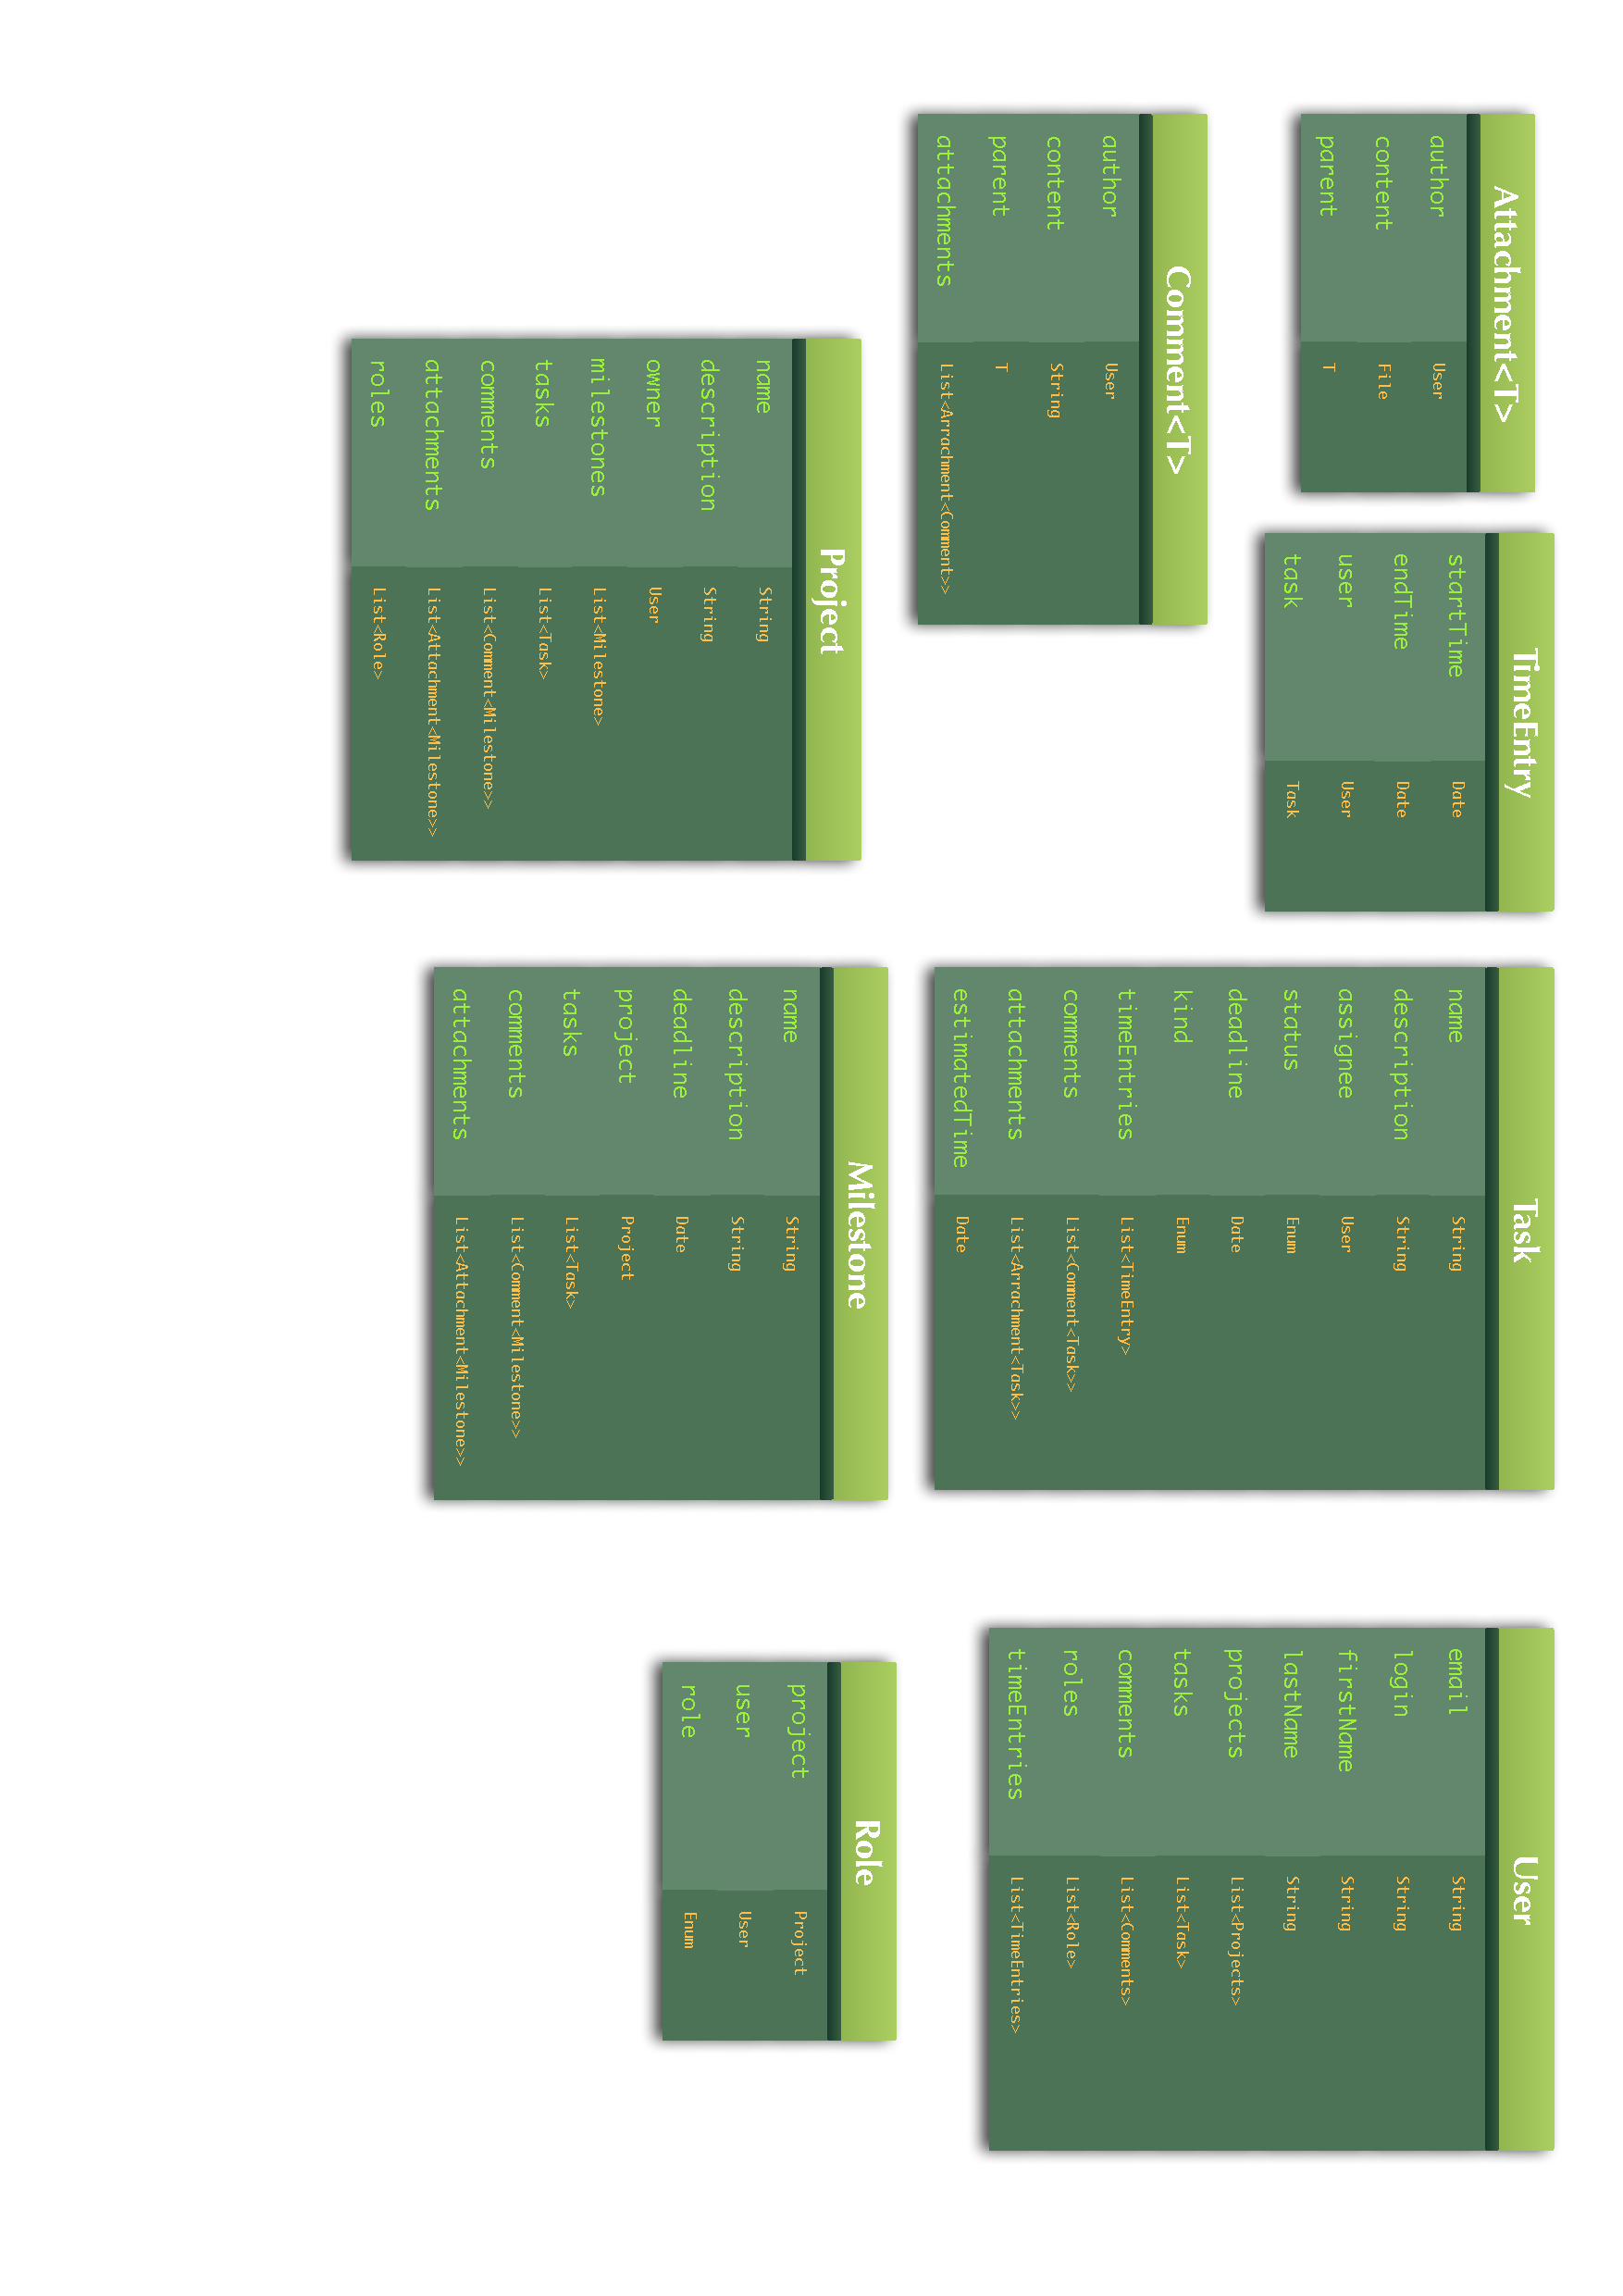
\includegraphics[width=\textwidth]{schemat.pdf}
      \caption{Model bazy danych}
    \end{center}
  \end{figure}

  \newpage

  \section{Testy wydajnościowe}
  \paragraph{}

  \subsection{Wydajność wyszukiwania}
  \paragraph{}
  Przeprowadzony test polegał na wyszukaniu 1 000 pojedynczych rekordów na podstawie parametru $id$ dla różnych wielkości bazy danych.


  \begin{longtable}{|c|c|c|}
    \hline
    $n$ &	$t [ms]$	& $n/t$ \\
    \hline
    100	& 251	  & 2,5100 \\
    200	& 463	  & 2,3150 \\
    400	& 926	  & 2,3150 \\
    800	& 1 863	& 2,3288 \\
    1600 & 3 894 & 2,4338 \\
    3200 & 7 942 & 2,4819 \\
    \hline
    \caption{Czas wyszukiwania w zależności od wielkości bazy danych}
  \end{longtable}

  \begin{figure}[H]
    \begin{center}
      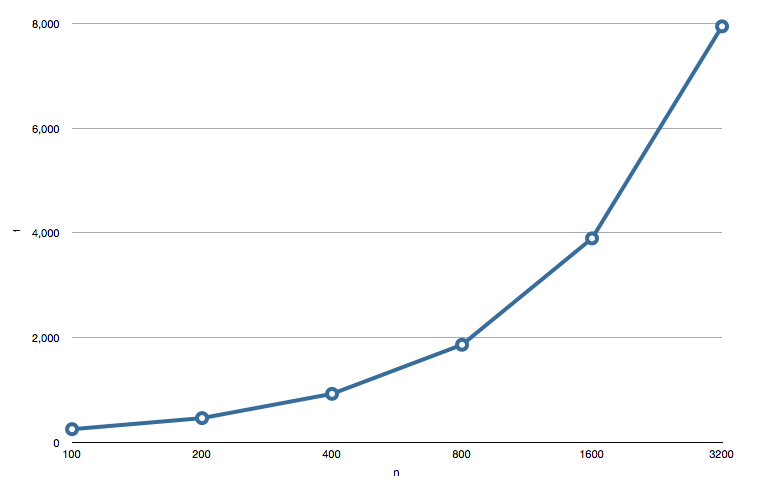
\includegraphics[width=\textwidth]{1.png}
      \caption{Czas wyszukiwania w zależności od wielkości bazy danych}
    \end{center}
  \end{figure}

  \paragraph{}
  Jak widać w Tabeli 1 oraz na Rysunku 1 czas wyszukiwania jest liniowo zależny od ilości rekordów w bazie. Wpływ na to ma algorytm wyszukiwania, który korzysta z przeglądu zupełnego wszystkich obiektów bazy danych.

  \newpage
  \subsection{Wydajność zapisu}
  \paragraph{}
  Zapis danych w obiektowej bazie danych NeoDatis dzieli sie na dwa etapy. Pierwszym etapem jest operacja \texttt{odb.store(obj)}, a kolejnym operacja \texttt{odb.commit()} przypominająca nieco operacje \texttt{COMMIT} znaną z operacji na transakcjach w relacyjnych bazach danych. Dodatkowo, w połączeniu klient-serwer używanym przez aplikacje dopiero operacja \texttt{odb.commit()} przesyła dane do serwera bazy danych. W związku z narzutem czasowym na transfer informacji po sieci zapisywanie i wysyłanie każdego obiektu osobno może okazać się mało wydajne.
Test polegał na zapisaniu (za pomocą \texttt{odb.store(obj)}) do bazy danych 10 000 obiektów w grupach po 1, 10, 100, 1 000 oraz 10 000 obiektów. Po zapisaniu grupy obiektów wywoływana była metoda \texttt{odb.commit()} odpowiedzialna za przesłanie zapisanych danych do serwera. Table 2 oraz Rysunek 2 prezentują wyniki testu.

  \begin{longtable}{|c|c|}
    \hline
    $n$ &	$t [ms]$ \\
    \hline
    1 & 1 313 \\
    10   & 526 \\
    100  & 349 \\
    1000 & 343 \\
    10000 &	475 \\
    \hline
    \caption{Czas zapisu w zależności od wielkości paczki}
  \end{longtable}


  \begin{figure}[H]
    \begin{center}
      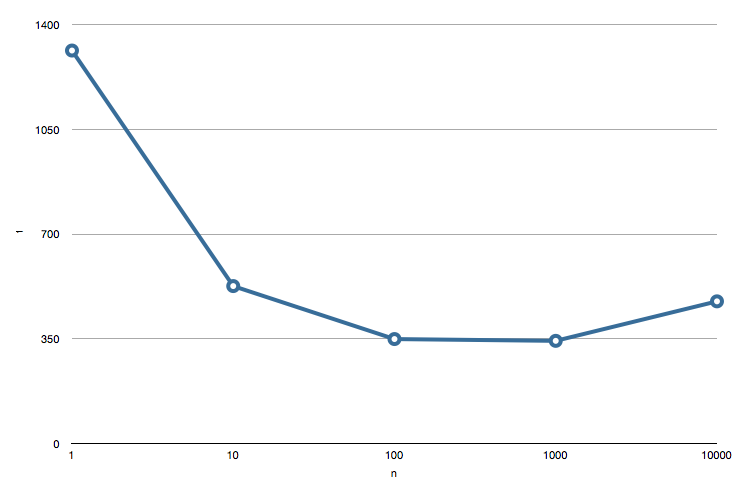
\includegraphics[width=\textwidth]{2.png}
      \caption{Czas zapisu w zależności od wielkości paczki}
    \end{center}
  \end{figure}

  \paragraph{}
  Po przeprowadzeniu testów okazało się, że najlepsze rezultaty daje zapisywanie obiektów w paczkach po 100 - 1 000 obiektów jednocześnie. Jednorazowe wysłanie 10 000 obiektów okazało się dłuższe, niż np. 10 razy po 1 000 obiektów.

  \newpage
  \section{Wnioski}
  \paragraph{}
  W porównaniu do relacyjnych baz danych bazy obiektowe nie są ograniczone przez tabele z danymi typu prostego (liczba, ciąg znaków, data) lecz pozwalają na trzymania danych dowolnych typów w dowolnie zagnieżdżonej strukturze. W łatwy sposób można przechować relacje jeden do wielu (za pomocą listy) czy wiele do wiele (za pomocą dwóch list). Z założenia obiektowych baz danych przechowywane obiekty nie wymagają specjalnego klucza głównego. W przypadku bazy danych NeoDatis działającej na maszynie wirtualnej Javy kluczami obiektów są wewnętrzne identyfikatory obiektów maszyny wirtualnej. Pozwala to na przeźroczyste przechowywanie danych obiektowych.

  \paragraph{}
  Wykorzystanie obiektowej bazy danych w aplikacji sieciowej pociąga za somą pewne konsekwencje. Ze względu na bezstanowość protokołu HTTP, wszysktie obiekty, na których mają być wykonywane operacja muszą posiadać niezmienny identyfikator, przesyłany jako część adresu URL lub w parametrach POST zapytania HTTP. Jest to równoznaczne ze sztucznym wprowadzeniem unikalnego identyfikatora dla każdego obiektu zapisanego w bazie danych. Obiektowa baza danych NeoDatis nie posiada mechanizmu automatycznej inkrementacji pola (\texttt{AUTO INCREMENT}). W związku z tym taką funkcjonalnośc należało napisać samemu. Przydzielenie nowego identyfikatora numerycznego ($id$) podczasu zapisu nowego obiektu sprowadza się do przeszukania całej bazy danych i wybranie maksymalnej wartości parametru $id$, a następnie przypisanie do nowego obiektu wartości o 1 większej. Taka operacja jest mało wydajna w porównaniu do podobnych mechanizmów w relacyjnych bazach danych.

  \paragraph{}
  W celu wykorzystania potencjału obiektowej bazy danych, należy też pamiętać, żeby przy relacjach uzupełniać dane po obu stronach relacji. Dla przykładu, przy relacji jeden do wielu w bazach relacyjnych wystarczy zapisać tylko identyfikator rekordu A w polu klucza obcego rekordu B. W obiektowej bazie danych należy przypisać referencje do obiektu A w obiekcie B, ale też dodać obiekt B do kolekcji obiektów typu B w obiekcie A. Bez zapisania obiektu B na liście zatraca się idea bazy obiektowej i wyszukiwanie elementów prowadza się do przeszukania całej bazy w poszukiwaniu obiektu o zadanym kluczu obcym.

\paragraph{}
  Ze względu na bezstanowość protokołu HTTP traci się wiele zalet obiektowych baz danych, a także zwiększa się czas odczytu i zapisu danych. Nie bez znaczenia jest konieczność implementacji własnych mechanizmów kontroli poprawności (unikalne identyfikatory, relacje).
  \paragraph{}
  Biorąc pod uwagę specyfikę i zasadę działania obiektowych baz danych, znajdą one szersze zastosowanie w aplikacjach desktopowych (wszędzie tam, gdzie można w prosty sposób połączyć interfejs użytkownika z modelem danych) niż w aplikacjach sieciowych opeartych o bezstanowy protokół HTTP.
\end{document}



